\documentclass[10pt]{article}
\usepackage{icmlko}

\icmlmeta{IP 파운데이션 월드모델}{292}{동률을 어떻게 깼나}{오늘 만든 축 여덟이 동률을 행 순서로 깨고 있었다 --- 고치니 새 도메인이 두 배로 좋아졌다}

\begin{document}

\twocolumn[
\icmlheader

\begin{abstract}
노트 291이 ``IP 조인을 넓히면 학습 상관이 $+$0.1392 $\to$ $+$0.2114 로
오른다''고 보고했다. 같은 것을 하네스 쪽 라벨로 다시 재니 부호가 안 맞아서
팠다. \textbf{lab 의 축과 레코드 원본이 다른 답을 냈다} --- 축 대 라벨은
학습 $+$0.1392 · 유보 $+$0.2042 인데 레코드의 \texttt{prior\_count} 대 라벨은
$+$0.0091 · $-$0.0087 이다. 그런데 둘의 상관은 $+$1.0000 이다. \textbf{같은
열인데 답이 다르면 동률이다.} 원인을 찾았다 --- 내가 오늘 쓴 \texttt{\_pct}
가 \texttt{argsort(argsort())} 로 백분위를 매기는데 그건 \textbf{동률을 행
순서로 깬다.} \texttt{prior\_count} 는 205행 중 \textbf{182행(89\%)이 0} 이고
행 순서가 \texttt{MKT-YYYY-NNNN} 이라 \textbf{연도와 $+$0.864} 다. 그래서
값이 전부 같은 182행 안에서 축이 라벨과 $+$0.1371 이 나왔다 --- \textbf{있지도
않은 정보를 축이 나르고 있었다.} 시장팝업 네 축의 진짜 값은 2 · 3 · 4 · 6개인데
\textbf{전부 205개로 펼쳐져} 있었다. \texttt{rankdata} 로 고치고 다시 쟀다.
\textbf{예상과 반대였다} --- 시장팝업 $\rho$ 가 \textbf{$+$0.1970 $\to$
$+$0.4051}, 치환 대비 \textbf{$z{=}2.02 \to 4.30$}($p$ 0.045 $\to$ $<$0.001)
이다. \textbf{인공물이 돕는 게 아니라 해치고 있었다} --- 값 여섯 개짜리 열을
205개로 펼치면 나무가 그 잡음(${\approx}$연도)에 갈라지고 유보에서 무너진다.
그러니 노트 284의 결론은 무너지는 게 아니라 \textbf{훨씬 강해진다.} 반면
노트 291의 ``조인 개선''은 \textbf{통째로 이 인공물이었다.}
\end{abstract}
]

\section{두 측정이 안 맞았다}

노트 291이 IP 조인을 넓혀 시장팝업의 \texttt{venue\_prominence}
(${=}$\texttt{ip\_history.prior\_count})가 학습 상관 $+$0.1392 $\to$ $+$0.2114
로 오르는 것을 보고했다. 하네스 쪽 라벨(내부 $+$ 시장 304건)로 같은 것을
재니 부호가 안 맞았다. 그래서 lab 의 축과 레코드 원본을 나란히 놨다.

\begin{center}\small
\begin{tabular}{lrr}
\hline
& 학습 & 유보 \\
\hline
lab 의 \texttt{venue\_prominence} & $+$0.1392 & $+$0.2042 \\
레코드의 \texttt{prior\_count} & $+$0.0091 & $-$0.0087 \\
\hline
\multicolumn{3}{l}{그런데 둘의 spearman ${=}$ \textbf{$+$1.0000}} \\
\hline
\end{tabular}
\end{center}

\textbf{같은 열이 같은 라벨과 다른 상관을 낼 수는 없다.} 단조 변환은 순위를
안 바꾼다. \emph{동률이 없다면.}

\section{argsort 가 동률을 행 순서로 깬다}

\begin{figure*}[t]
\centering
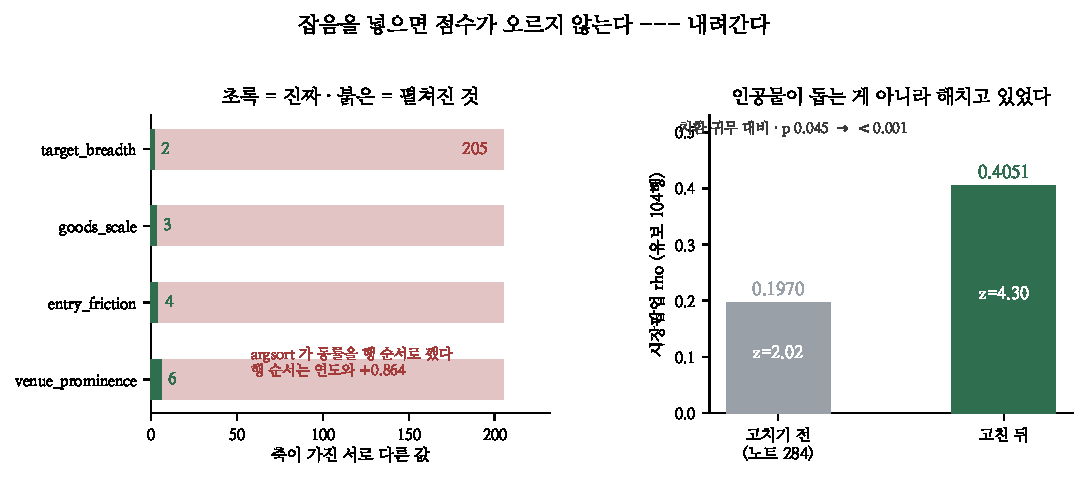
\includegraphics[width=\textwidth]{figs/tie.pdf}
\caption{왼쪽 --- 시장팝업 네 축이 실제로 가진 값의 수와 펼쳐진 수.
오른쪽 --- 고치기 전후의 도메인 $\rho$ 와 치환 대비 $z$.}
\end{figure*}

오늘 쓴 \texttt{\_pct} 는 이랬다.

\begin{center}\small
\begin{verbatim}
r = np.argsort(np.argsort(x))
out[ok] = r / max(len(x) - 1, 1)
\end{verbatim}
\end{center}

\texttt{argsort} 를 두 번 하면 동률에도 \textbf{서로 다른} 순위가 붙고, 그
순서는 \textbf{입력 배열의 인덱스 순서}다.

\begin{center}\small
\begin{tabular}{lr}
\hline
\texttt{prior\_count} 가 0 인 행 & \textbf{182 / 205 (89\%)} \\
행 순서와 연도의 상관 & \textbf{$+$0.864} \\
\hline
\textbf{그 182행 안에서 축과 라벨} & \textbf{$+$0.1371} \\
\hline
\end{tabular}
\end{center}

\textbf{값이 전부 같은 182행 안에서 축이 라벨을 예측한다.} 그 정보는 자료에
없다 --- 파일 이름이 \texttt{MKT-2023-\ldots} 에서 \texttt{MKT-2026-\ldots}
로 가고 라벨에 연도 추세가 있어서 생긴 것이다.

네 축이 다 그랬다.

\begin{center}\small
\begin{tabular}{lrr}
\hline
축 & 진짜 값 & 펼쳐진 값 \\
\hline
\texttt{target\_breadth} & 2 & 205 \\
\texttt{goods\_scale} & 3 & 205 \\
\texttt{entry\_friction} & 4 & 205 \\
\texttt{venue\_prominence} & 6 & 205 \\
\hline
\end{tabular}
\end{center}

\paragraph{고침} \texttt{rankdata}(동률에 평균 순위)로 바꿨다.
\texttt{ingest/market\_axes.py} 와 \texttt{lab/popaxes.py} 둘 다 오늘 내가
쓴 것이다. 확인: 동률 182행의 축 값이 \textbf{정확히 하나}(상수)가 되고,
축의 서로 다른 값이 \textbf{6 ${=}$ 원본과 같고}, 축 대 라벨이 원본과 일치한다
($+$0.0091 · $-$0.0087).

\section{예상과 반대였다}

인공물을 걷어내면 점수가 내려갈 줄 알았다. \textbf{올랐다.}

\begin{center}\small
\begin{tabular}{lrr}
\hline
& 고치기 전 & 고친 뒤 \\
\hline
\textbf{시장팝업 $\rho$} & $+$0.1970 & \textbf{$+$0.4051} \\
치환 귀무 & $-$0.0029$\pm$0.099 & $-$0.0003$\pm$0.094 \\
\textbf{$z$} & $+$2.02 & \textbf{$+$4.30} \\
$p$ & 0.045 & \textbf{$<$0.001} \\
\hline
기존 아홉 & \multicolumn{2}{c}{순 $-$0.0007 · 진짜 0개} \\
출처 가드 & \multicolumn{2}{c}{통과} \\
\hline
\end{tabular}
\end{center}

\textbf{잡음을 넣으면 점수가 오르는 게 아니라 내려간다.} 값 여섯 개짜리 열을
205개로 펼치면 나무가 그 사이 어디서나 갈라질 수 있고, 갈라 봐야 학습에서만
맞는 연도 무늬라 유보에서 무너진다. 노트 259가 잰 것의 반대 방향이다 ---
그때는 \emph{쓸모 있는} 열이 뿌리 근처를 차지해 다른 도메인을 밀어냈고,
여기서는 \emph{쓸모없는} 열이 제 도메인을 밀어냈다.

\paragraph{그래서 노트 284가 강해진다} 열한 번째 도메인을 열 때 $\rho{=}0.197$
에 $z{=}2.02$($p{=}0.045$)라 ``아슬아슬하다''고 적었다. 진짜 값은
\textbf{0.4051 · $z{=}4.30$} 이다. 활성 축 다섯으로 그렇다 --- 웹툰이 열여덟
축으로 0.45 를 내는 판에서다.

\paragraph{그리고 노트 291은 통째로 틀렸다} ``IP 조인을 넓히면 학습 상관이
$+$0.1392 $\to$ $+$0.2114'' --- 그 두 수가 \textbf{둘 다 이 인공물}이다.
고친 뒤 진짜 값은 $+$0.0091(학습) · $-$0.0087(유보)이고, 조인을 넓혀도
거기서 안 움직인다. \textbf{조인을 넓힌 것 자체는 여전히 옳다}(오탐을 걷어내고
잇는 IP 가 23 $\to$ 40) --- 다만 그 이득을 잰 자가 망가져 있었다.

\section{어디까지 번졌나}

\begin{center}\small
\begin{tabular}{ll}
\hline
노트 & 정정 \\
\hline
284 & $\rho$ 0.197 $\to$ \textbf{0.405} · $z$ 2.02 $\to$ 4.30 \\
285 & 오염된 바탕 위에서 잰 것 --- 재측정 중 \\
291 & 학습 상관 개선은 \textbf{전부 인공물} \\
276$\sim$287 & \texttt{popaxes} 도 같은 \texttt{\_pct} 였으나 \\
& 청력 문턱 때문에 전부 정확히 0.0000 --- \textbf{결론 불변} \\
\hline
\end{tabular}
\end{center}

마지막 줄이 다행이다. 팝업 전용 축들은 나무가 아예 안 썼으므로(노트 276 ·
281 · 287) 오염된 채로도 0.0000 이었고, 그 노트들의 결론은 안 바뀐다.

\paragraph{남은 것}
\begin{center}\small
\begin{tabular}{ll}
\hline
갈래 & 왜 \\
\hline
\texttt{mkt\_cat} 재측정 & 노트 285를 고친 바탕에서 \\
다른 \texttt{\_pct} 감사 & \texttt{trendaxes} 는 \texttt{rankdata} 라 안전 \\
가드로 만들까 & ``값보다 순위가 많은 축''을 잡으면 된다 \\
만화↔웹툰 174건 & 별칭 사전의 진짜 값어치는 여기다 \\
\hline
\end{tabular}
\end{center}

\paragraph{규약} \textbf{동률이 많은 열을 백분위로 바꿀 때는 동률을 어떻게
깨는지 본다.} \texttt{argsort(argsort())} 는 편해 보이지만 \textbf{입력 순서를
값에 섞는다.} 그리고 \textbf{두 측정이 안 맞으면 셋째를 찾는다} --- 축과
원본이 상관 $+$1.0000 인데 라벨과의 상관이 다르다는 모순이 없었으면 이걸
못 찾았다. 오늘 아침 노트 274가 ``저장된 점수를 실행 가로질러 빼지 말라''로
시작했는데, 저녁에는 \textbf{같은 실행 안에서 두 경로가 안 맞는 것}이 열쇠였다.

\end{document}
